\subsection{Multi environment Reinforcement Learning from Verifiable Rewards}
\label{subsec:RLVR}
We employ a unified RLVR stage, training on all environments simultaneously. We find that this results in stable gains across all benchmarks throughout training, while single environment training often results in un-recoverable degradation of other benchmarks. We do two stages of such RLVR: one immediately after SFT and one after RLHF.
\subsubsection{Environments}

% \todo{Soumye. Highly suggest we give some numbers regarding the scale of each of the envs, e.g. if it is the competitive coding, how many samples with how many unit test in total? Additionally, if you want to sell the scale, we can talk about in total how many samples have been used through the RLVR stage (this could even be before we talk about details about each envs).}

\textbf{Competition Math.} We train on the DAPO \citep{yu2025dapo} and SkyWorks math \citep{he2025skywork} datasets. These datasets have 17K and 104K tasks respectively.

\textbf{Competition Coding.} We use competitive coding problems from \citet{ahmad2025opencodereasoning}. We limit the number of unit tests to 50 in order to reduce verification time. This filtering leaves us with 22K tasks.

\textbf{Question Answering.} We train on a variety of difficult multiple choice datasets focusing on STEM domains. Here the questions and answers are generated based on information from reference documents. This dataset has with 135K tasks.

\textbf{Structured Outputs.} We train \ourmodel to have strong JSON schema adherence capabilities. We utilized NeMo Data Designer \citep{nemo-data-designer} to create the seed dataset for RL. We start by constructing (JSON schema, document) pairs conditioned on diverse topics using Qwen3-235B-A22B-Instruct-2507 \citep{yang2025qwen3technicalreport}. We then utilized these pairs to create RL prompts by taking the model to summarize the document according to the schema.  To ensure high syntactic validity, the pipeline enforced strict complexity controls and applied rejection sampling, while simultaneously varying instruction difficulty and phrasing to maximize input diversity. This pipeline produces 9K tasks.

In the RL stage, a positive reward is given when the output matches the exact schema constraints, and no reward is given otherwise. For simplicity, we do not add a reward for the semantic content of the output.

\textbf{Instruction Following.} We use two instruction following environments during the training. The first environment is similar to the IFEval style environment used in \citet{bercovich2025llamanemotronefficientreasoningmodels}, but with refreshed constraints from the IFBench training set \citep{pyatkin2025generalizing}. We create 46K tasks for this environment.

The second environment uses LLM as a judge to verify whether or not the agent has followed complex instructions in multi-turn settings, where the instructions may be quite subtle. This environment is inspired by the Multi-Challenge benchmark \citep{deshpande2025multichallenge}. We create 3K total tasks for it.

\textbf{Long Context.}
We generate challenging long-context QA pairs using Qwen3-235B-A22B-Thinking-2507 \citep{yang2025qwen3technicalreport}, drawing from a subset of our pre-training mixture designed for multi-document synthesis. Each question is required to reference at least five documents, with the total input limited to 32k tokens. We employ Qwen3-235B-A22B-Instruct-2507 \citep{yang2025qwen3technicalreport} as the LLM judge to evaluate the model's rollouts. This dataset contains 12K tasks.

\textbf{Agentic Tool Use.} We use two environments to improve tool use capabilities. The first is Workplace Assistant, a multi-step verifiable tool-calling setup adapted from Styles \citep{Styles2024WorkBench} that was also used in Nemotron 2 Nano \citep{nemotronnanov2}. This is a tool use - multi step agentic environment that tests the agent's ability to execute tasks in a workplace setting. Workplace Assistant contains a sandbox environment with five databases, 26 tools, and 690 tasks. These tasks represent common business activities, such as sending emails, scheduling meetings, etc. The correctness is verified through executing the tool calls issued by the agent and comparing it to the ground truth database state. 

The second environment is a Multi-turn conversational agent environment. It tests an agent's tool-calling and proactive asking capability. Comprising approximately 1K tasks, this environment simulates complex banking scenarios like assisting customers with unblocking a credit card or solving account disputes. The correctness of the agent's actions is automatically verified by executing the tool calls it issues and comparing the resulting database state against the predefined ground truth.



\subsubsection{Data Mixture and Curriculum}
We begin by profiling all reinforcement learning (RL) tasks using our supervised fine-tuning (SFT) checkpoint. To focus training on challenging cases, we filter out samples where the SFT checkpoint already achieves a 100\% pass rate. We then adopt the curriculum training method introduced in~\citet{bercovich2025llamanemotronefficientreasoningmodels}, which dynamically adjusts task difficulty throughout training.

In each batch, we maintain a fixed ratio of samples across different domains. For each domain, we model the target pass-rate distribution as a Gaussian function, shifting from high pass-rate (easier) samples early in training to low pass-rate (harder) samples later. The target mean of Gaussian distribution decreases linearly throughout training steps. Within each batch, samples from different domains are shuffled. This Gaussian sampling strategy prevents overfitting to either overly easy or overly difficult examples, ensuring a balanced learning progression. 

This approach enables a controlled and gradual increase in task difficulty while preserving domain diversity and ensuring efficient batch composition. Figure~\ref{fig:pass_rate} illustrates how sample difficulty evolves over the course of RL training. Once training progress plateaus, we re-profile the tasks using the best RL checkpoint and construct a new curriculum to further refine performance.

\begin{figure}[ht]
    \centering
    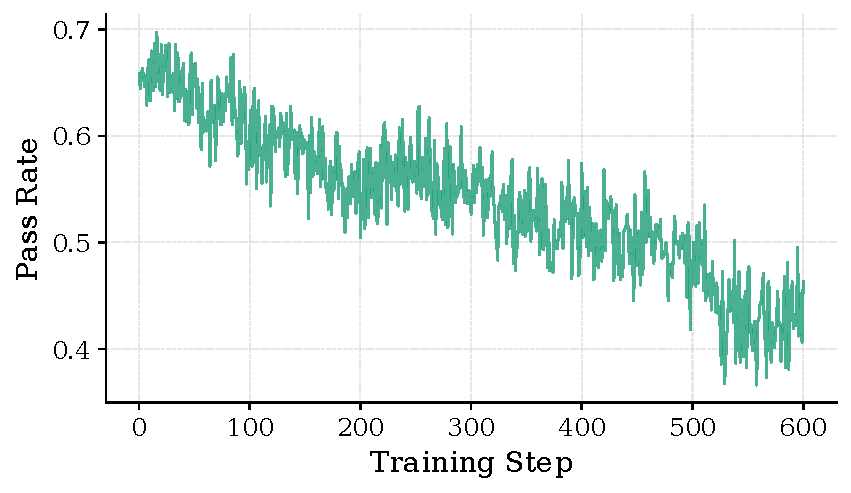
\includegraphics[width=0.6\textwidth]{figures/pass_rate.pdf}
    \caption{Batch-wise pass rates across the RL curriculum.}
    \label{fig:pass_rate}
\end{figure}

We compare curriculum sampling against random sampling using an intermediate SFT checkpoint, maintaining identical domain ratios in both cases. As shown in Figure~\ref{fig:curriculum_ablation}, curriculum sampling ensures stable learning across multiple domains throughout training. In contrast, random sampling biases the model toward easier tasks, preventing it from effectively learning more challenging ones.

\begin{figure}[ht]
    \centering
    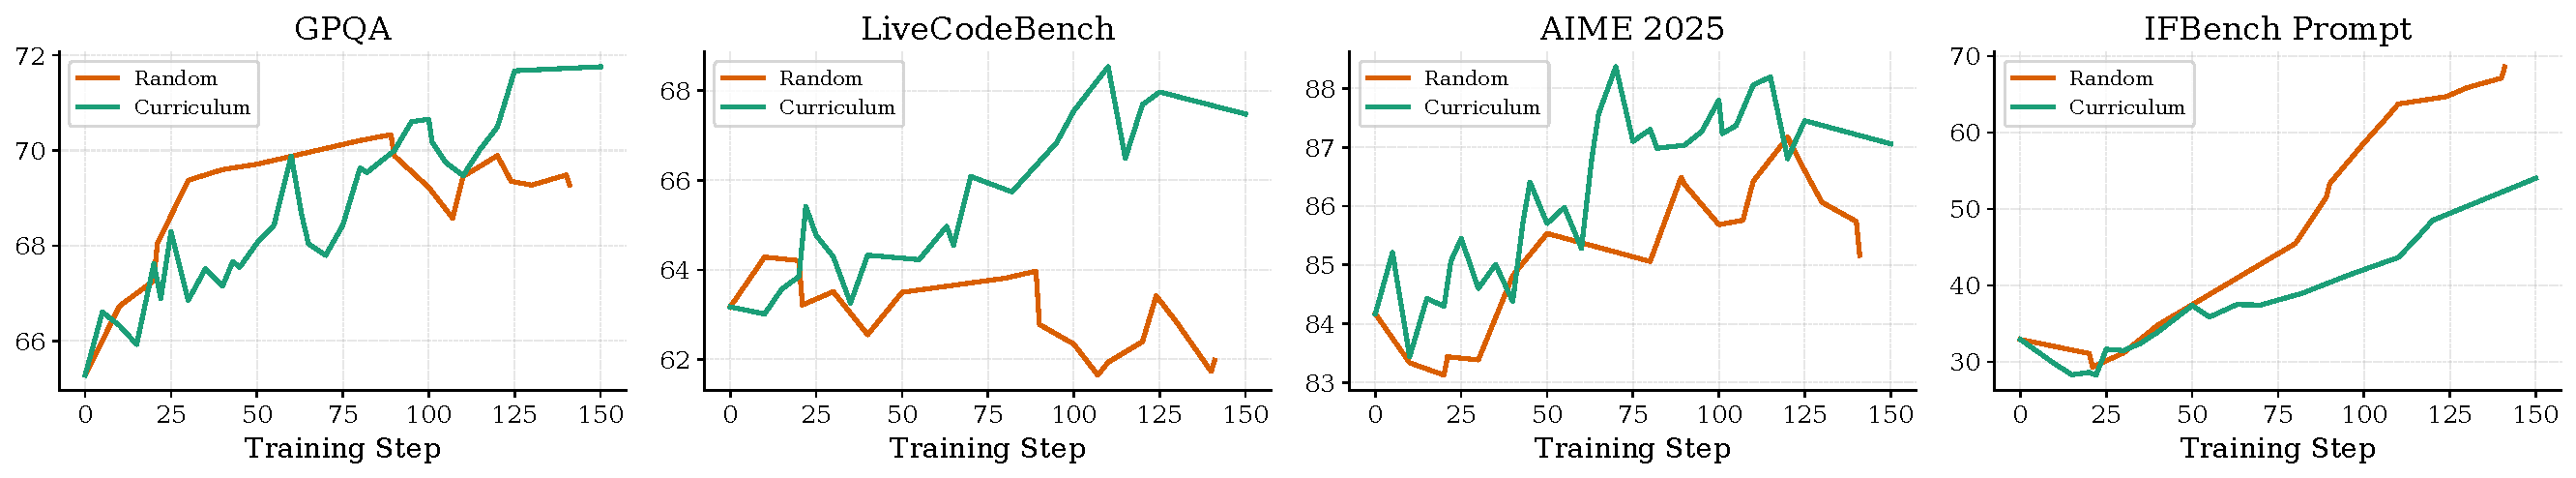
\includegraphics[width=\textwidth]{figures/rlvr_compare_curriculum.pdf}
    \caption{Comparison between curriculum sampling and random sampling.}
    \label{fig:curriculum_ablation}
\end{figure}

\subsubsection{Surpassing SFT with RLVR}

Recent works have demonstrated that supervised fine-tuning (SFT) alone on small models can achieve strong performance~\citep{ahmad2025opencodereasoning,deepseekai2025deepseekr1incentivizingreasoningcapability}. In this study, we investigate whether RLVR can outperform a heavily fine-tuned SFT baseline. As illustrated in Figure~\ref{fig:surpass_sft_with_rlvr}, we compare the accuracy of model during RLVR training with two SFT checkpoints: 
\begin{itemize} 
\item SFT1: Our initial RLVR starting point, fine-tuned for approximately 3 epochs. 
\item SFT2: A heavily fine-tuned checkpoint, trained to full convergence (approximately 5 epochs). \end{itemize} 
Our results show that even with relatively short training, RLVR consistently exceeds  or matches the accuracy of the heavily fine-tuned SFT model across all evaluated domains.
\begin{figure}[ht]
    \centering
    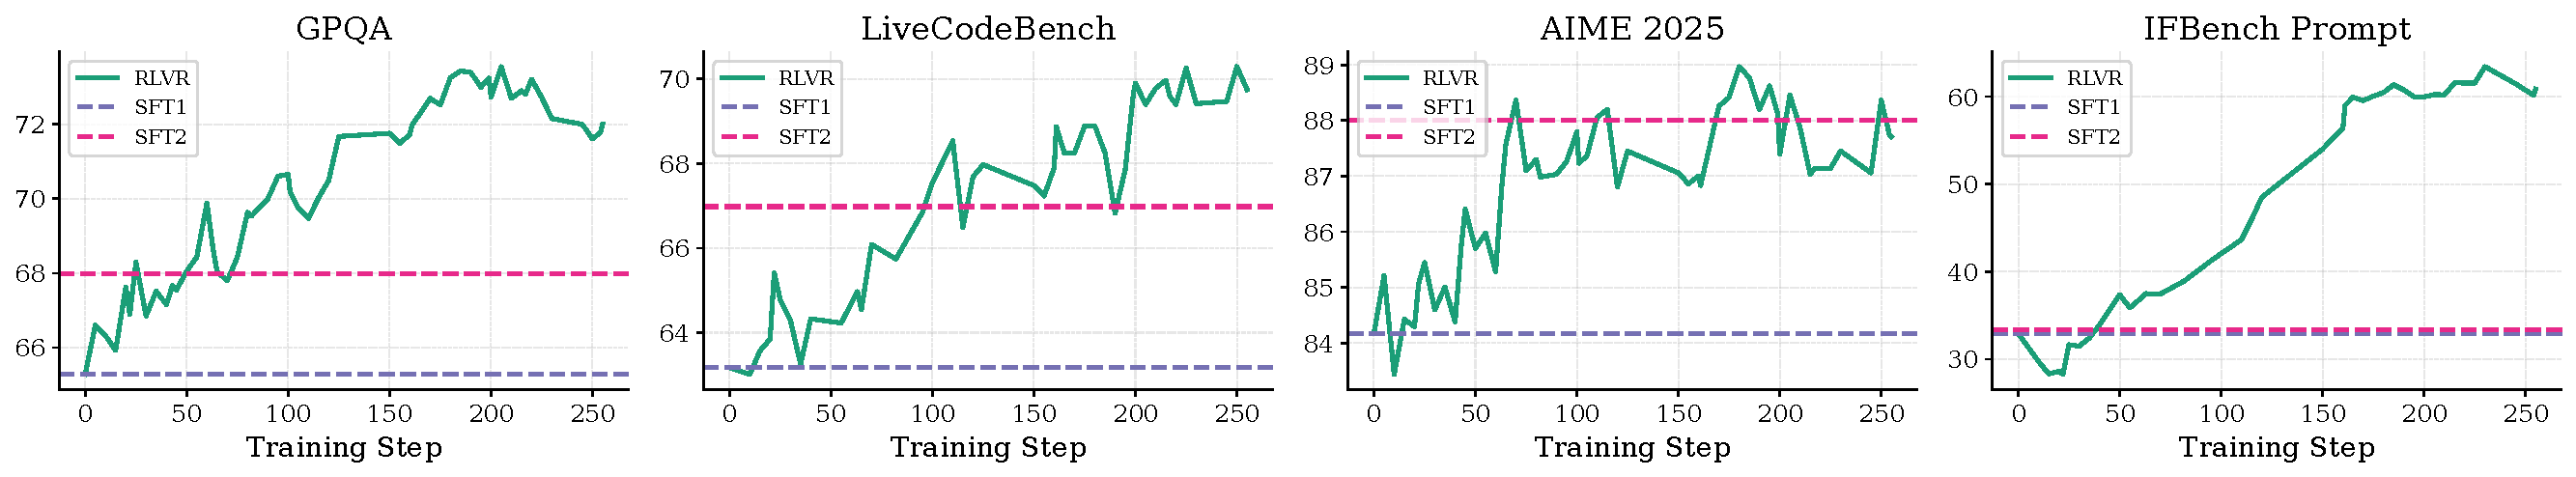
\includegraphics[width=\textwidth]{figures/rlvr_surpass_sft.pdf}
    \caption{RLVR surpasses or matches heavily fine-tuned SFT model across all evaluated domains.}
    \label{fig:surpass_sft_with_rlvr}
\end{figure}


\subsubsection{Infrastructure}
\label{subsubsection:RLinfra}

RL at the frontier of model post-training is currently defined by scaling up to an increasing diversity of tasks or environments designed for the model to learn increasingly general capabilities.
Scaling RL to many environments requires a high-performance, extensible, and standardized interface for coordinating between rollouts and training.
To address the scaling performance and extensibility challenges using one standard framework, we adopt NeMo Gym \citep{nemo-gym} and NeMo RL \citep{nemo-rl} for enabling large-scale RL on many different environments/verifiers.

NeMo Gym is based on the abstraction of \emph{servers}.
There are three core varieties of servers in Gym: (1) \emph{agents}, (2) \emph{models}, and (3) \emph{resources}.
An \emph{agent} server implements the rollout kernel of a RL environment.
A \emph{model} server wraps an inference engine such as vLLM \citep{kwon2023efficientmemorymanagementlarge} to provide a prompt-response API, and also carefully preserves token and inference log-prob data and metadata required for RL.
A \emph{resource} server provides a verification API for computing rewards from a given rollout.

Our Nemotron Nano 3 RLVR experiments were all based on an integrated infrastructure of NeMo RL and NeMo Gym:
NeMo RL acts as the RL training loop controller, using Megatron-Core \citep{shoeybi2020megatronlmtrainingmultibillionparameter} for model training at scale, and routing all rollouts through NeMo Gym and vLLM.

\subsubsection{Algorithm}
\label{sec:rl-algo}
We train \ourmodel using synchronous GRPO with masked importance sampling to mitigate training-inference misalignment \citep{Shao2024DeepSeekMath, team2025every, yao2025offpolicy}. We use 128 prompts per step and use 16 generations per prompt. We train with a batch size of 2048, making our updates on-policy. To further stabilize training we also freeze the MoE router weights. We employ the aux-loss-free load balancing approach and keep updating expert bias~\citep{wang2024auxiliary}. 

Our entire training run is done with a maximum generation length of 49K. We use overlong filtering \citep{yu2025dapo}, which we find boosts performance on reasoning intensive benchmarks.


% \subsubsection{SFT Initialization}
% \todo{Peter, Alex?: Early, medium, late SFT ckpt}


\begin{figure}[ht]
    \centering
    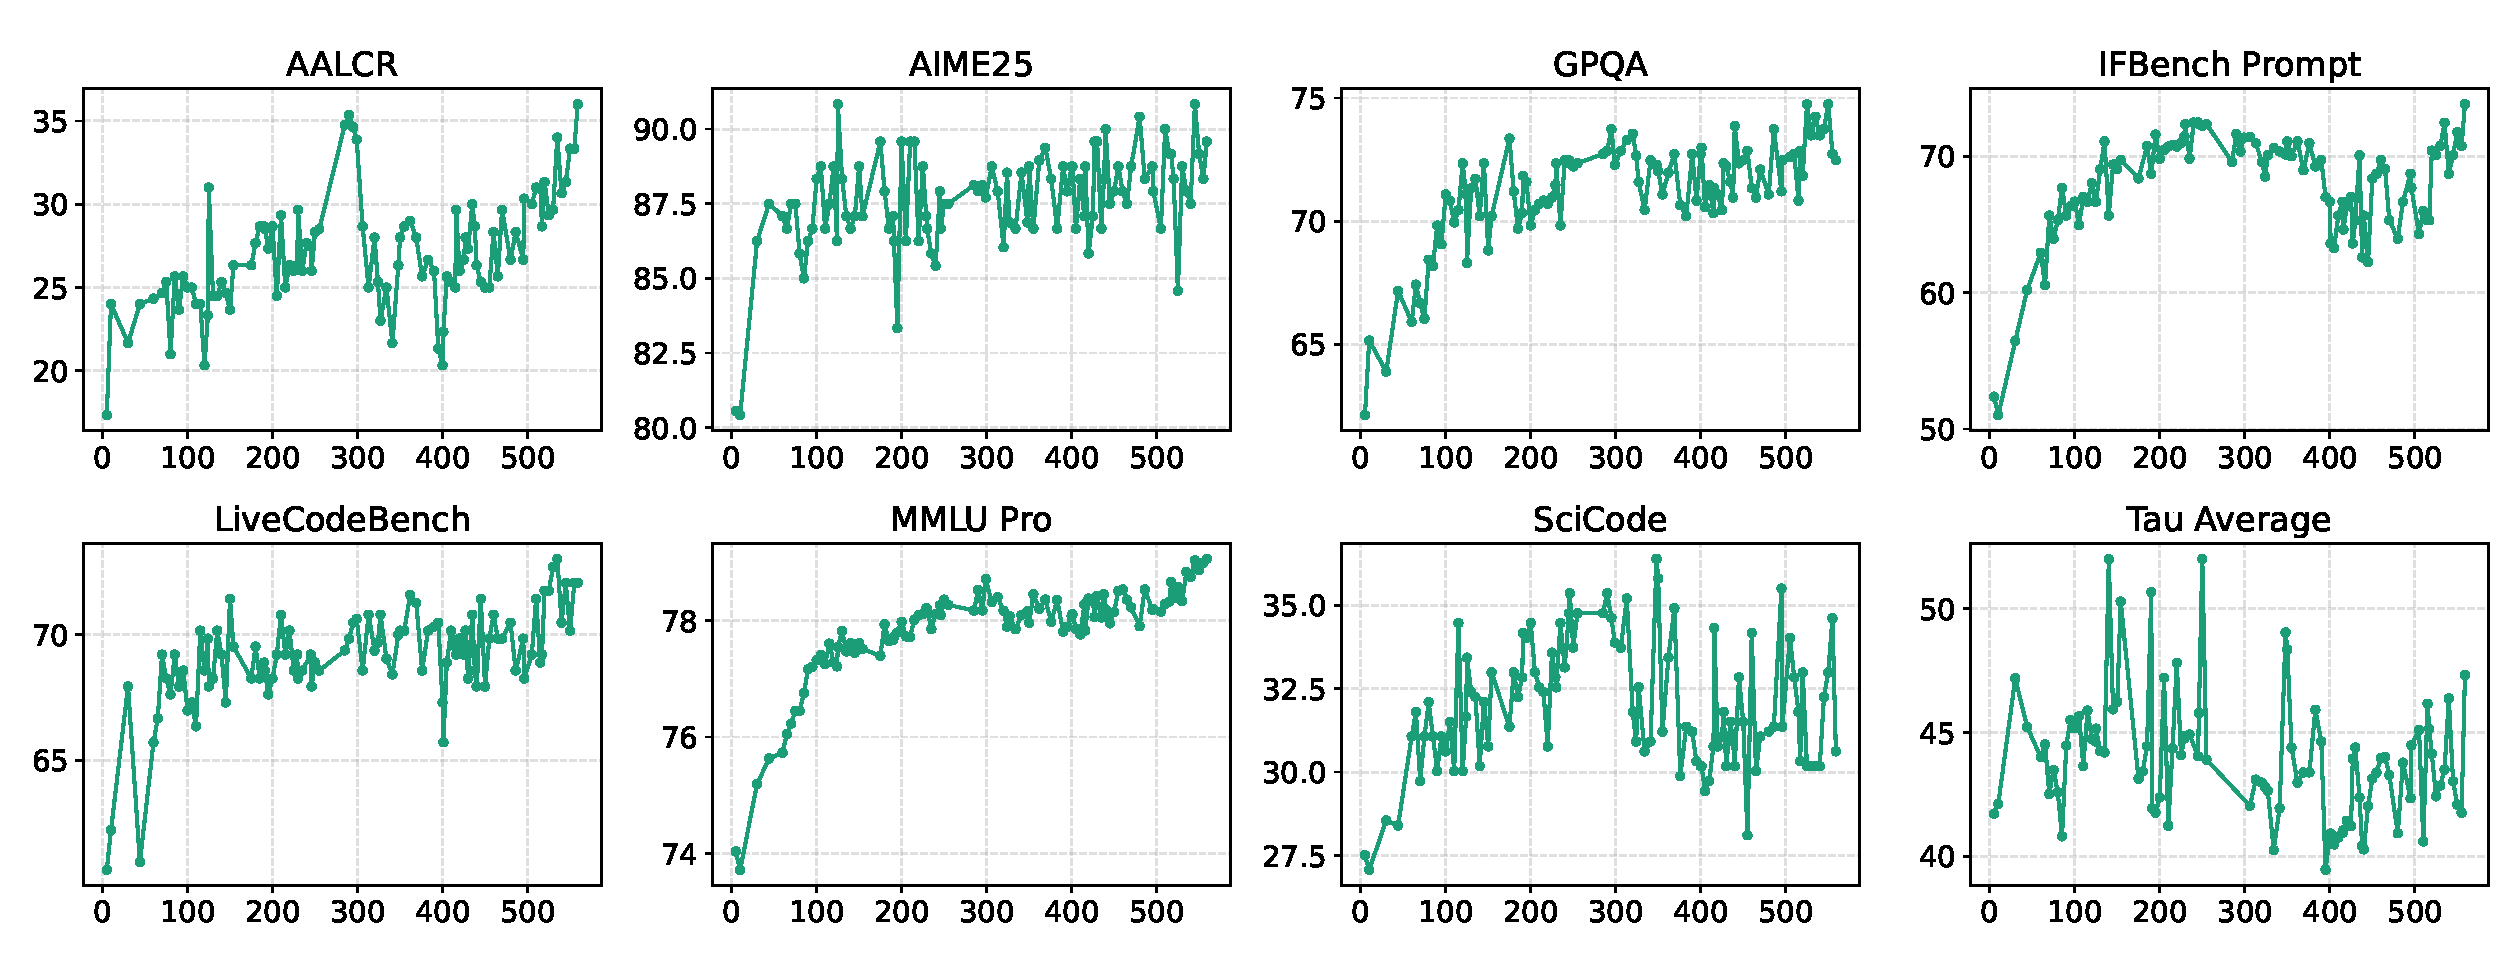
\includegraphics[width=\textwidth]{figures/rl_progress_concat.pdf}
    \caption{Benchmark performance throughout RL training.}
    \label{fig:rl_progress}
\end{figure}